\chapter{Vergelijkend onderzoek}
\label{ch:vergelijkend onderzoek}

In dit hoofdstuk wordt het vergelijkend onderzoek besproken. Training- en testdata zijn verzameld en de testapplicatie is klaar om gebruikt te worden. Eerst zullen er voor elk framework drie modellen getraind worden, onderverdeeld per categorie van producten. 
Alle gebruikte afbeeldingen, getrainde modellen en testapplicatie zijn terug te vinden op Github\footnote{\url{https://github.com/Jeremy-vdw/Bachelorproef-Productherkenning/tree/master/documentatie}}.

\section{Frameworks trainen}
\label{sec:Tensorflow}

\subsection{Tensorflow}
\label{ssec:Tensorflow}

Een \acrshort{CNN} opnieuw trainen met tensorflow is eenvoudig, al vraagt het toch geringe kennis over machine learning en python. Om het tensorflow model te gebruiken in een iOS applicatie vraagt heel wat meer moeite. Het tensorflow model moet geconverteerd worden naar het coreML formaat en dat is niet van zelfsprekend. Aangezien het aantal trainingsafbeeldingen beperkt is, kan het proces uitgevoerd worden door de processor en is er geen hulp van een grafische kaart nodig. Standaard worden tensorflow processen uitgevoerd door alleen de \acrshort{CPU}, maar er kan wel ingesteld worden dat ook de \acrshort{GPU} de processen verwerkt.  De training en conversie wordt uitgelegd met betrekking tot de kleine producten, het proces verliep echter volledig simultaan voor de middelgrote en grote producten.  

\subsubsection{Model trainen}
\label{sssec:Model trainen}

Na het installeren van Tensorflow kon het proces gestart worden. Op de officiële github repository van Tensorflow\footnote{\url{https://github.com/tensorflow/tensorflow}} bevindt zich de code \textit{'retrain.py'}, de code die ervoor zorgt dat het een bestaand model opnieuw getraind kan worden. Door volgend commando in de terminal uit te voeren kon Tensorflow starten met het trainen van het model voor kleine producten.

\codefragment{code/commando.txt}{Code voor het trainen van een model met Tensorflow }

Het bestand \textit{'retrain.py'} werd uitgevoerd door python. \textit{'-\phantom{}-bottleneck\_dir'} is de map waar de bottlenecks van de trainingsafbeeldingen moeten worden opgeslagen. Tensorflow gebruikt de term bottleneck voor de output van de voorlaatste laag. \textit{'-\phantom{}-output\_graph'} is een verwijzing naar het bestand waar het model in moet worden bewaard, waar de bijhorende labels worden opgeslagen wordt meegegeven door  \textit{'-\phantom{}-output\_labels'}.  \textit{'-\phantom{}-image\_dir'} is de map die wordt gebruikt om het model te trainen, in die map bevindt zich de trainingsdata. 

\subsubsection{Model converteren}
\label{sssec:Model converteren}

Het tensorflow moest worden omgezet naar een mlmodel. Daarvoor werd een converter, Tfcoreml\footnote{\url{https://github.com/tf-coreml/tf-coreml}}, gebruikt. Eerst moest de naam van de laatste laag, de softmax-laag, en de input naam verkregen werden. De softmax-laag geeft de waarschijnlijkheid dat de input gelijk is aan een klasse, voor elke klasse in het model terug. Om dit te achterhalen werd er gebruik gemaakt van Netron\footnote{\url{https://github.com/lutzroeder/Netron}} een open source programma die een neuraal netwerk visualiseert en zo duidelijk maakt wat de input en output van het netwerk is. 

Uit de visuele voorstelling kon verstaan worden dat de input de naam \textit{'Placeholder'} heeft en dat het een drie dimensionale array met diepte drie is. De breedte en hoogte moet 299 pixels zijn. Verder werd afgeleid dat de output van het netwerk als naam \textit{'final\_result'} heeft. Figuur \ref{fig:visualisatienetron} geeft een beeld hoe de naam van de in- en output laag verkregen is. Hierdoor was er voldoende informatie om het Tensorflow model om te zetten naar een CoreML model. Wanneer tfcoreml was geïnstalleerd, werd onderstaande code gebruikt om het model voor kleine producten te converteren. 


\begin{figure}[!ht]
    \centering
    \begin{subfigure}{.5\textwidth}
      \centering
      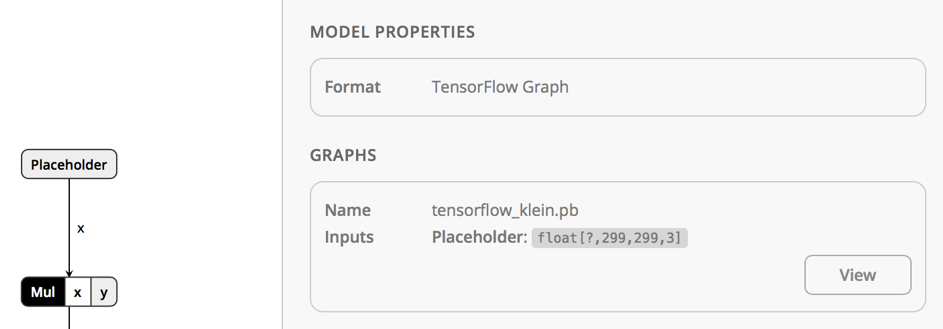
\includegraphics[width=.95\linewidth]{img/input_netron.png}
      \caption{De input laag}
      \label{fig:sub1}
    \end{subfigure}%
    \begin{subfigure}{.5\textwidth}
      \centering
      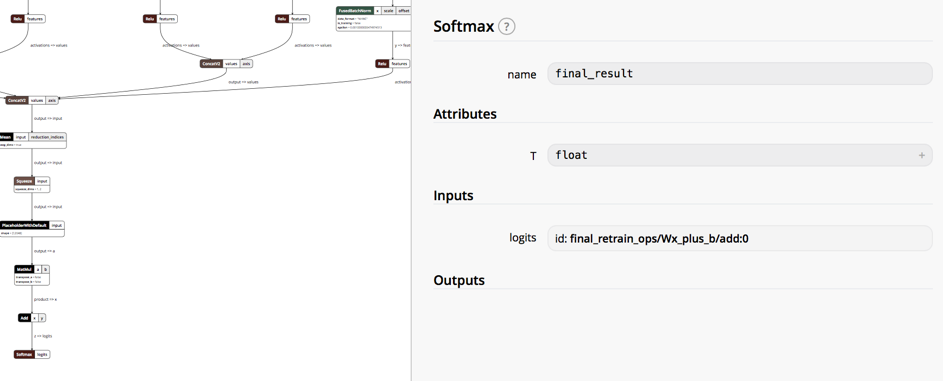
\includegraphics[width=.95\linewidth]{img/output_netron.png}
      \caption{De output laag}
      \label{fig:sub2}
    \end{subfigure}
    \caption{Visualisatie van het model m.b.v. Netron }
    \label{fig:visualisatienetron}
\end{figure}

\newpage
\codefragment{code/convertor.py}{Code voor conversie m.b.v. Tfcoreml}

\textit{'tf\_model\_path'} en \textit{'mlmodel\_path'} zijn een verwijzing naar het pad van het Tensorflow model en van het nieuwe mlmodel. \textit{'output\_feature\_names'} is de naam van de uitvoerlaag die verkregen is door Netron. De naam en de vorm van de input moet worden meegegeven aan \textit{'input\_name\_shape\_dict'}. Om de input te veranderen van een drie dimensionale array naar een afbeelding wordt variabele \textit{'image\_input\_names'} meegegeven. Tenslotte wordt het pad naar de labels aangeduid met \textit{'class\_labels'}. De laatste vier regels dienen om de afbeelding te bewerken alvorens het als input gebruikt wordt voor het neurale netwerk. Dit is op aanraden van Google om betere resultaten te behalen \autocite{hackermoon2}. 

\subsection{Turi Create}
\label{ssec:Turi Create}

Wanneer Turi Create gebruikt wordt om een eigen classificatiemodel te creëren wordt er ook een \acrshort{CNN} opnieuw getraind. Zoals eerder vermeld vraagt het toepassen van Turi Create naar eigen zeggen van Apple amper kennis over machine learning. In vergelijking met Tensorflow vraagt Turi Create meer Python in de vorm van het aantal lijnen code. Om het model dat Turi Create produceert om te zetten naar CoreML is er echter één lijn code nodig en is het dus zeer eenvoudig. Net zoals Tensorflow vereist Turi Create geen grafische kaart om een model te trainen, maar ook bij dit framework kan \acrshort{GPU}-ondersteuning worden ingeschakeld. Het trainen en converteren van het model wordt uitgelegd voor middelgrote producten. De zelfde acties werden ondernomen voor kleine en grote producten

\newpage
\subsubsection{Model trainen en converteren}
\label{sssec:Model trainen en converteren}

\codefragment{code/convertor.py}{Trainen en converteren van het model met Turi Create}

Met \textit{'url'} wordt er verwezen naar de map waar de trainingsdata zich bevindt. Daarna wordt de trainingsdata geanalyseerd door Turi Create en omgezet naar een array en opgeslaan in \textit{'data'}. Om de trainingsdata te voorzien van de juiste labels bevat de array \textit{‘labels’} alle nodige namen van labels. De functie \textit{‘get\_label’} vergelijkt de naam van de map waarin een afbeelding zich bevindt met de labels, als deze overeenstemmen dan krijgt een afbeelding overeenkomstig label toegewezen. Nadat elke afbeelding heeft juiste label heeft gekregen kan er met behulp van Turi Create een model ontwikkeld worden. In de laatste regel wordt het model gemakkelijk omgezet naar het CoreML-formaat.

\subsection{Turi Create}
\label{ssec:Turi Create}

Dit framework toepassen voor een eigen classificatiemodel vraagt echter geen enkele kennis van Python of machine learning. Het framework komt met een volledige web interface en is zeer eenvoudig te gebruiken.
In vergelijking met de twee vorige frameworks is er voor dit framework geen installatie of dergelijke nodig. Het framework kan gebruikt worden op de officiële website\footnote{\url{https://www.customvision.ai}}. Om het model te exporteren naar het CoreML-formaat wordt er tevens geen enkele kennis vereist. Met enkele klikken is het model omgezet. 

\subsubsection{Model trainen en converteren}
\label{sssec:Model trainen en converteren}

Na het aanmaken van een nieuw project op de website van Custom Vision, kon er eenvoudig afbeeldingen per product geüpload worden. Elk product werd benoemd met een andere tag. Nadat alle productafbeeldingen op de website stonden kon het model getraind worden door simpelweg op de button ‘train’ te klikken. In figuur \ref{fig:customvision} is een voorbeeld te zien van Custom Vision die als input de trainingsdata voor grote producten had. Hetzelfde gebeurde voor kleine en middelgrote producten.

\begin{figure}
    \centering
        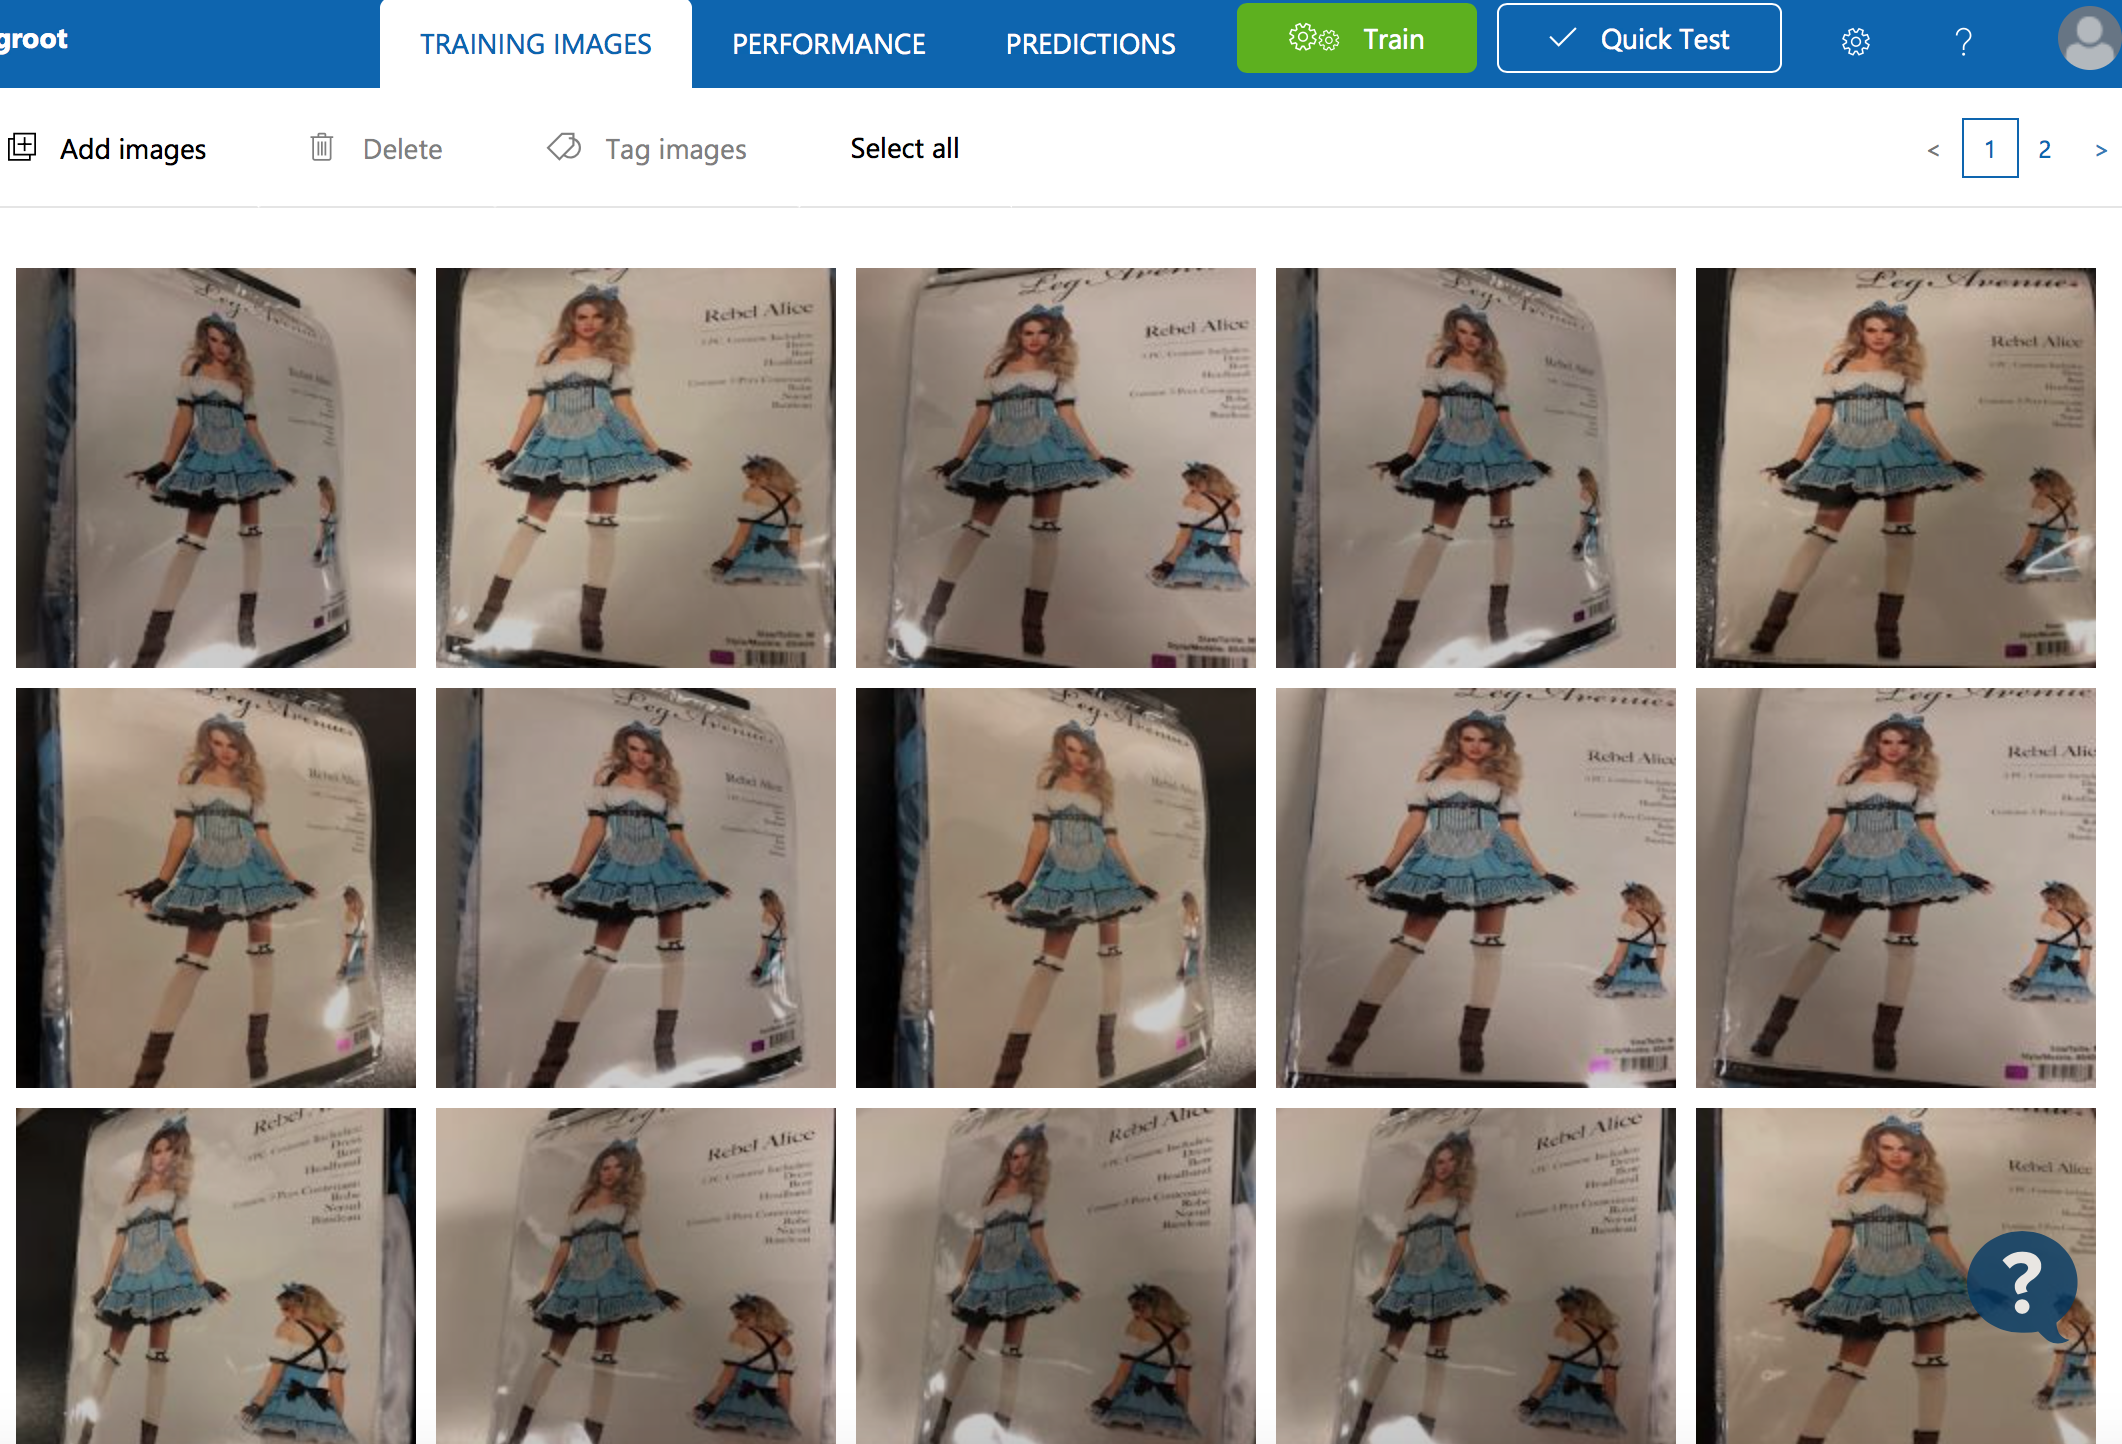
\includegraphics[width=0.8\textwidth]{img/customvision.png}
    \caption{Voorbeeld van Custom Vision}
    \label{fig:customvision}
  \end{figure}

Na de training van het model werd er een overzicht van de nauwkeurigheid van het getrainde model gegeven. Vervolgens kon op de button ‘export’ geklikt worden om het mlmodel te verkrijgen.

\section{Resultaten vergelijken}
\label{sec:Resultaten vergelijken}

\subsection{Kleine producten}
\label{ssec:Kleine producten}

Om te frameworks te vergelijken voor kleine producten werd de testdata uit figuur \ref{fig:testklein} gebruikt. Het viel op dat Tensorflow enkel oog had voor één specifiek product. Voor nagenoeg alle testafbeeldingen kreeg het label ‘neon feathers’ de hoogste waarschijnlijkheid. In tegenstelling tot Tensorflow waren Turi Create en Custom Vision betrouwbaarder. Op 30 testafbeeldingen konden deze frameworks respectievelijk 24 en 29 afbeeldingen juist classificeren. Tensorflow kon slechts aan 11 afbeeldingen de juiste klasse toewijzen. In figuur \ref{fig:grafiekkleineproducten} worden de resultaten grafisch voorgesteld.

\begin{figure}[ht!]
  \centering
      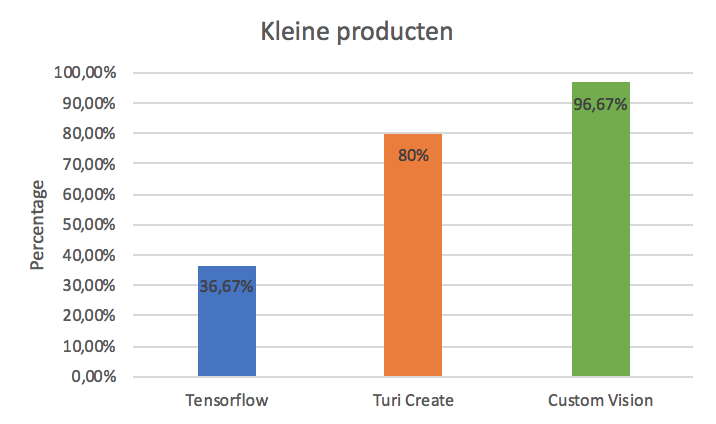
\includegraphics[width=0.8\textwidth]{img/grafiekkleineproducten.png}
  \caption{Grafische weergave juist geclassificeerde testafbeeldingen in percentage per framework voor kleine producten}
  \label{fig:grafiekkleineproducten}
\end{figure}

\subsection{Middelgrote producten}
\label{ssec:Middelgrote producten}

Met de testdata uit figuur \ref{fig:testmiddel} voor middelgrote producten kon hetzelfde vastgesteld worden voor Tensorflow als bij kleine producten.  Ook bij deze producten herkende het framework vrijwel altijd dezelfde klasse in een afbeelding. Bijna elke afbeelding had het label ‘amber’ als opperste waarschijnlijkheid. Tensorflow labelde 13 van de 30 testafbeeldingen correct. Bij deze groep producten scoorden Turi Create en Custom Vision evengoed. Elk konden ze 26 afbeeldingen keurig classificeren.  In grafische voorstelling wordt getoond in figuur \ref{fig:grafiekmiddelproducten}.

\begin{figure}[ht!]
  \centering
      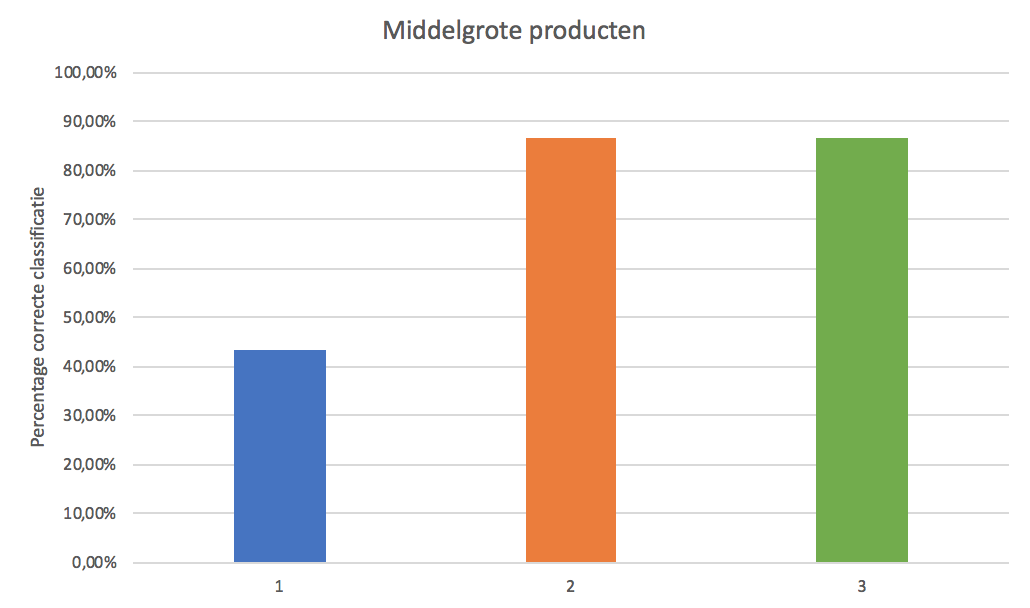
\includegraphics[width=0.8\textwidth]{img/grafiekmiddelproducten.png}
  \caption{Grafische weergave juist geclassificeerde testafbeeldingen in percentage per framework voor middelgrote producten}
  \label{fig:grafiekmiddelproducten}
\end{figure}

\subsection{Grote producten}
\label{ssec:Grote producten}

In tegenstelling tot voorgaande groepen producten kon Tensorflow met de testdata uit figuur \ref{fig:testgroot} voor grote producten aan meer producten de juiste klasse toewijzen. Tensorflow kon grotendeels de testafbeeldingen van ‘hypnoticAlice’ en ‘rebelAlice’ juist classificeren. Aan 19 van de 30 testfoto’s werd het juiste label toegewezen met Tensorflow. Net als bij de kleine en middelgrote producten scoorden Turi Create en Custom Vision hoog. Turi Create classificeerde 25 afbeeldingen correct. In figuur \ref{fig:grafiekgroteproducten} worden de resultaten gevisualiseerd.

\begin{figure}[ht!]
  \centering
      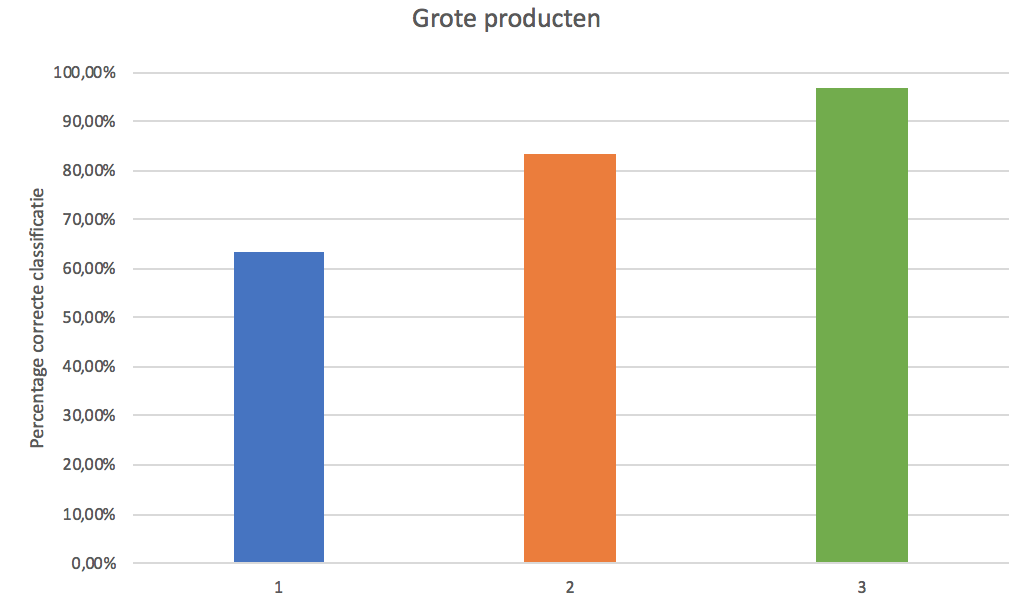
\includegraphics[width=0.8\textwidth]{img/grafiekgroteproducten.png}
  \caption{Grafische weergave juist geclassificeerde testafbeeldingen in percentage per framework voor grote producten}
  \label{fig:grafiekgroteproducten}
\end{figure}

\section{Besluit}
\label{sec:Besluit}

Na het vergelijken van de frameworks voor de verschillende groottes van producten overtrof Custom Vision steeds de andere twee frameworks. Naast het meest nauwkeurige framework is Custom Vision ook het minst complexe.

Opvallend was dat Tensorflow veel beter scoorde bij grote producten dan bij kleine producten. Dit heeft wellicht als reden dat bij de testdata van kleine producten veel meer achtergrond te zien was dan bij de testafbeeldingen van grote producten.  Zou Tensorflow toegepast worden om een eigen productclassificatie model te creëren voor een bedrijf of winkel, dan zou het toestel genoeg moeten inzoomen op het product om herkend te worden door Tensorflow.

Aangezien de resultaten van Turi Create en Custom Vision weinig verschilden ten opzichte van elkaar, zou een ontwikkelaar met kennis van machine learning en python ook voor Turi Create kunnen kiezen. 

  